
        \documentclass[spanish, 11pt]{exam}

        %These tell TeX which packages to use.
        \usepackage{array,epsfig}
        \usepackage{amsmath, textcomp}
        \usepackage{amsfonts}
        \usepackage{amssymb}
        \usepackage{amsxtra}
        \usepackage{amsthm}
        \usepackage{mathrsfs}
        \usepackage{color}
        \usepackage{multicol, xparse}
        \usepackage{verbatim}


        \usepackage[utf8]{inputenc}
        \usepackage[spanish]{babel}
        \usepackage{eurosym}

        \usepackage{graphicx}
        \graphicspath{{../img/}}



        \printanswers
        \nopointsinmargin
        \pointformat{}

        %Pagination stuff.
        %\setlength{\topmargin}{-.3 in}
        %\setlength{\oddsidemargin}{0in}
        %\setlength{\evensidemargin}{0in}
        %\setlength{\textheight}{9.in}
        %\setlength{\textwidth}{6.5in}
        %\pagestyle{empty}

        \let\multicolmulticols\multicols
        \let\endmulticolmulticols\endmulticols
        \RenewDocumentEnvironment{multicols}{mO{}}
         {%
          \ifnum#1=1
            #2%
          \else % More than 1 column
            \multicolmulticols{#1}[#2]
          \fi
         }
         {%
          \ifnum#1=1
          \else % More than 1 column
            \endmulticolmulticols
          \fi
         }
        \renewcommand{\solutiontitle}{\noindent\textbf{Sol:}\enspace}

        \newcommand{\samedir}{\mathbin{\!/\mkern-5mu/\!}}

        \newcommand{\class}{1º Bachillerato}
        \newcommand{\examdate}{\today}

        \newcommand{\tipo}{A}


        \newcommand{\timelimit}{50 minutos}



        \pagestyle{head}
        \firstpageheader{
\includegraphics[width=0.2\columnwidth]{header_left}}{\textbf{Departamento de Matemáticas\linebreak \class}\linebreak \examnum}{
\includegraphics[width=0.1\columnwidth]{header_right}}
        \runningheader{\class}{\examnum}{Página \thepage\ of \numpages}
        \runningheadrule

        \newcommand{\examnum}{41 - Estadística Unidimensional}
        \begin{document}
        \begin{questions}
        \question autoevaluacion1 - Se realiza una encuesta a un grupo de 20 personas acerca del número 
                  de veces que acuden al cine a lo largo de un año, obteniéndose los siguientes resultados:4 2 6 8 3 4 3 5 7 1 3 4 5 7 2 2 1 3 4 5
        \begin{multicols}{1} 
        \begin{parts} \part[1] Realiza una tabla de frecuencias  \begin{solution}   \begin{tabular}{rrrrrrr}
\hline
   x\_i &   f\_i &   F\_i &   h\_i &   H\_i &   \%\_i &   \%A\_i \\
\hline
     1 &     2 &     2 &  0.1  &  0.1  &    10 &     10 \\
     2 &     3 &     5 &  0.15 &  0.25 &    15 &     25 \\
     3 &     4 &     9 &  0.2  &  0.45 &    20 &     45 \\
     4 &     4 &    13 &  0.2  &  0.65 &    20 &     65 \\
     5 &     3 &    16 &  0.15 &  0.8  &    15 &     80 \\
     6 &     1 &    17 &  0.05 &  0.85 &     5 &     85 \\
     7 &     2 &    19 &  0.1  &  0.95 &    10 &     95 \\
     8 &     1 &    20 &  0.05 &  1    &     5 &    100 \\
\hline
\end{tabular}   \end{solution} \part[1] Realiza un diagrama de barras y un polígono de frecuencias  \begin{solution}   \\ 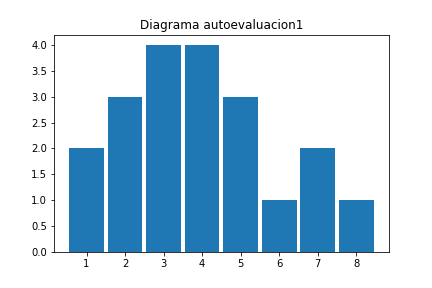
\includegraphics[width=1\columnwidth]{autoevaluacion1}   \end{solution} \part[1] Calcular los parámetros de centralización  \begin{solution}   {'media': 3.95, 'mediana': 4.0, 'moda': ModeResult(mode=array([3]), count=array([4]))}   \end{solution} \part[1] Calcular los parámetros de posición P70, Q1, Q3, D4  \begin{solution}   {'P70': 5.0, 'Q1': 2.75, 'Q3': 5.0, 'D4': 3.0}   \end{solution} \part[1] Calcular los parámetros de dispersión  \begin{solution}   {'rango': 7, 'varianza': 3.747500000000001, 'desviación típica': 1.93584606826059, 'coeficiente variación': 0.490087612217872}   \end{solution}
        \end{parts}
        \end{multicols}
        \question p089e01 - Las calificaciones de un grupo de 34 alumnos han sido: 9 6 5 0 1 5 7 9 10 7 5 1 2 5 7 6 3 4 6 8 8 6 4 4 6 5 3 5 7 7 8 7 2 2
        \begin{multicols}{1} 
        \begin{parts} \part[1] Realiza una tabla de frecuencias  \begin{solution}   \begin{tabular}{rrrrrrr}
\hline
   x\_i &   f\_i &   F\_i &       h\_i &       H\_i &      \%\_i &      \%A\_i \\
\hline
     0 &     1 &     1 & 0.0294118 & 0.0294118 &  2.94118 &   2.94118 \\
     1 &     2 &     3 & 0.0588235 & 0.0882353 &  5.88235 &   8.82353 \\
     2 &     3 &     6 & 0.0882353 & 0.176471  &  8.82353 &  17.6471  \\
     3 &     2 &     8 & 0.0588235 & 0.235294  &  5.88235 &  23.5294  \\
     4 &     3 &    11 & 0.0882353 & 0.323529  &  8.82353 &  32.3529  \\
     5 &     6 &    17 & 0.176471  & 0.5       & 17.6471  &  50       \\
     6 &     5 &    22 & 0.147059  & 0.647059  & 14.7059  &  64.7059  \\
     7 &     6 &    28 & 0.176471  & 0.823529  & 17.6471  &  82.3529  \\
     8 &     3 &    31 & 0.0882353 & 0.911765  &  8.82353 &  91.1765  \\
     9 &     2 &    33 & 0.0588235 & 0.970588  &  5.88235 &  97.0588  \\
    10 &     1 &    34 & 0.0294118 & 1         &  2.94118 & 100       \\
\hline
\end{tabular}   \end{solution} \part[1] Realiza un diagrama de barras y un polígono de frecuencias  \begin{solution}   \\ 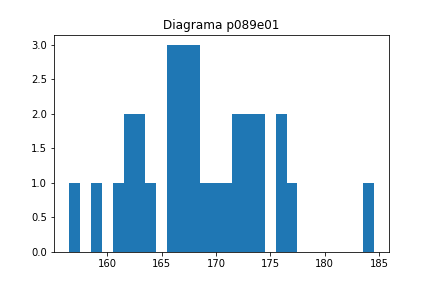
\includegraphics[width=1\columnwidth]{p089e01}   \end{solution} \part[1] Calcular los parámetros de centralización  \begin{solution}   {'media': 5.294117647058823, 'mediana': 5.5, 'moda': ModeResult(mode=array([5]), count=array([6]))}   \end{solution} \part[1] Calcular los parámetros de posición P70, Q1, Q3, D4  \begin{solution}   {'P70': 7.0, 'Q1': 4.0, 'Q3': 7.0, 'D4': 5.0}   \end{solution} \part[1] Calcular los parámetros de dispersión  \begin{solution}   {'rango': 10, 'varianza': 6.031141868512111, 'desviación típica': 2.45583832295860, 'coeficiente variación': 0.463880572114402}   \end{solution}
        \end{parts}
        \end{multicols}
        \question p089e02 - En un grupo de personas de 1º de Bachillerato hemos preguntado por el número medio de días que
                    practican deporte al mes. Las respuestas han sido las siguientes:16 11 17 12 10 5 1 8 10 14 15 20 10 3 8 10 2 5 12 6 16 7 6 16 10 3 3 9 4 12
        \begin{multicols}{1} 
        \begin{parts} \part[1] Realiza una tabla de frecuencias  \begin{solution}   \begin{tabular}{rrrrrrr}
\hline
   x\_i &   f\_i &   F\_i &       h\_i &       H\_i &      \%\_i &      \%A\_i \\
\hline
     1 &     1 &     1 & 0.0333333 & 0.0333333 &  3.33333 &   3.33333 \\
     2 &     1 &     2 & 0.0333333 & 0.0666667 &  3.33333 &   6.66667 \\
     3 &     3 &     5 & 0.1       & 0.166667  & 10       &  16.6667  \\
     4 &     1 &     6 & 0.0333333 & 0.2       &  3.33333 &  20       \\
     5 &     2 &     8 & 0.0666667 & 0.266667  &  6.66667 &  26.6667  \\
     6 &     2 &    10 & 0.0666667 & 0.333333  &  6.66667 &  33.3333  \\
     7 &     1 &    11 & 0.0333333 & 0.366667  &  3.33333 &  36.6667  \\
     8 &     2 &    13 & 0.0666667 & 0.433333  &  6.66667 &  43.3333  \\
     9 &     1 &    14 & 0.0333333 & 0.466667  &  3.33333 &  46.6667  \\
    10 &     5 &    19 & 0.166667  & 0.633333  & 16.6667  &  63.3333  \\
    11 &     1 &    20 & 0.0333333 & 0.666667  &  3.33333 &  66.6667  \\
    12 &     3 &    23 & 0.1       & 0.766667  & 10       &  76.6667  \\
    14 &     1 &    24 & 0.0333333 & 0.8       &  3.33333 &  80       \\
    15 &     1 &    25 & 0.0333333 & 0.833333  &  3.33333 &  83.3333  \\
    16 &     3 &    28 & 0.1       & 0.933333  & 10       &  93.3333  \\
    17 &     1 &    29 & 0.0333333 & 0.966667  &  3.33333 &  96.6667  \\
    20 &     1 &    30 & 0.0333333 & 1         &  3.33333 & 100       \\
\hline
\end{tabular}   \end{solution} \part[1] Realiza un diagrama de barras y un polígono de frecuencias  \begin{solution}   \\ 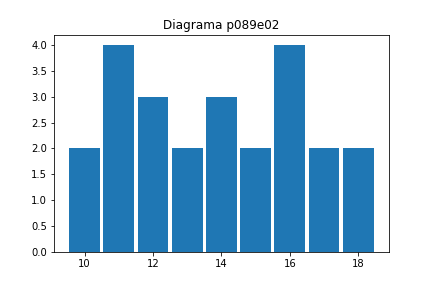
\includegraphics[width=1\columnwidth]{p089e02}   \end{solution} \part[1] Calcular los parámetros de centralización  \begin{solution}   {'media': 9.366666666666667, 'mediana': 10.0, 'moda': ModeResult(mode=array([10]), count=array([5]))}   \end{solution} \part[1] Calcular los parámetros de posición P70, Q1, Q3, D4  \begin{solution}   {'P70': 12.0, 'Q1': 5.25, 'Q3': 12.0, 'D4': 8.0}   \end{solution} \part[1] Calcular los parámetros de dispersión  \begin{solution}   {'rango': 19, 'varianza': 24.232222222222227, 'desviación típica': 4.92262351010335, 'coeficiente variación': 0.525546993961212}   \end{solution}
        \end{parts}
        \end{multicols}
        \question p089e03 - Estos datos reflejan el tiempo, en minutos, que tardan en llegar a su centro escolar varios alumnos. 10 15 11 11 14 14 11 14 17 11 17 15 10 16 12 12 13 16 13 16 18 12 18 16
        \begin{multicols}{1} 
        \begin{parts} \part[1] Realiza una tabla de frecuencias  \begin{solution}   \begin{tabular}{rrrrrrr}
\hline
   x\_i &   f\_i &   F\_i &       h\_i &       H\_i &      \%\_i &      \%A\_i \\
\hline
    10 &     2 &     2 & 0.0833333 & 0.0833333 &  8.33333 &   8.33333 \\
    11 &     4 &     6 & 0.166667  & 0.25      & 16.6667  &  25       \\
    12 &     3 &     9 & 0.125     & 0.375     & 12.5     &  37.5     \\
    13 &     2 &    11 & 0.0833333 & 0.458333  &  8.33333 &  45.8333  \\
    14 &     3 &    14 & 0.125     & 0.583333  & 12.5     &  58.3333  \\
    15 &     2 &    16 & 0.0833333 & 0.666667  &  8.33333 &  66.6667  \\
    16 &     4 &    20 & 0.166667  & 0.833333  & 16.6667  &  83.3333  \\
    17 &     2 &    22 & 0.0833333 & 0.916667  &  8.33333 &  91.6667  \\
    18 &     2 &    24 & 0.0833333 & 1         &  8.33333 & 100       \\
\hline
\end{tabular}   \end{solution} \part[1] Realiza un diagrama de barras y un polígono de frecuencias  \begin{solution}   \\ 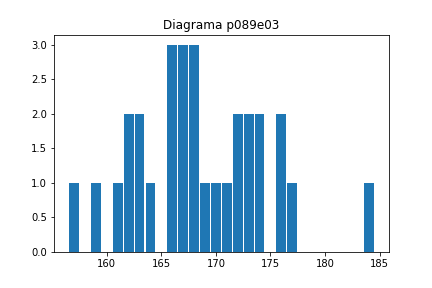
\includegraphics[width=1\columnwidth]{p089e03}   \end{solution} \part[1] Calcular los parámetros de centralización  \begin{solution}   {'media': 13.833333333333334, 'mediana': 14.0, 'moda': ModeResult(mode=array([11]), count=array([4]))}   \end{solution} \part[1] Calcular los parámetros de posición P70, Q1, Q3, D4  \begin{solution}   {'P70': 16.0, 'Q1': 11.75, 'Q3': 16.0, 'D4': 13.0}   \end{solution} \part[1] Calcular los parámetros de dispersión  \begin{solution}   {'rango': 8, 'varianza': 6.222222222222221, 'desviación típica': 2.49443825784929, 'coeficiente variación': 0.180320837916816}   \end{solution}
        \end{parts}
        \end{multicols}
        \question p089e03b - La altura en cm de 30 alumnos de un curso son:174 157 168 166 169 168 173 184 176 171 172 168 
                  167 162 162 163 166 166 167 167 
                  174 159 170 172 173 164 161 163 176 177
        \begin{multicols}{1} 
        \begin{parts} \part[1] Realiza una tabla de frecuencias  \begin{solution}   \begin{tabular}{rrrrrrr}
\hline
   x\_i &   f\_i &   F\_i &       r\_i &       R\_i &      \%\_i &      \%A\_i \\
\hline
 157.5 &     2 &     2 & 0.0666667 & 0.0666667 &  6.66667 &   6.66667 \\
 162.5 &     6 &     8 & 0.2       & 0.266667  & 20       &  26.6667  \\
 167.5 &    10 &    18 & 0.333333  & 0.6       & 33.3333  &  60       \\
 172.5 &     8 &    26 & 0.266667  & 0.866667  & 26.6667  &  86.6667  \\
 177.5 &     3 &    29 & 0.1       & 0.966667  & 10       &  96.6667  \\
 182.5 &     1 &    30 & 0.0333333 & 1         &  3.33333 & 100       \\
\hline
\end{tabular}   \end{solution} \part[1] Realiza un diagrama de barras y un polígono de frecuencias  \begin{solution}   \\ 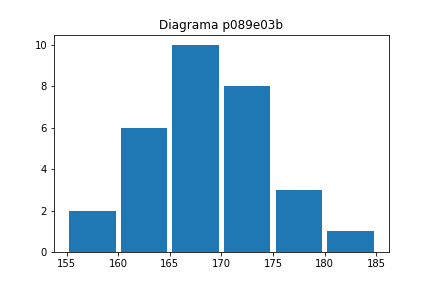
\includegraphics[width=1\columnwidth]{p089e03b}   \end{solution} \part[1] Calcular los parámetros de centralización  \begin{solution}   {'media': 168.66666666666666, 'mediana': 167.5, 'moda': ModeResult(mode=array([167.5]), count=array([10]))}   \end{solution} \part[1] Calcular los parámetros de posición  \begin{solution}   {'Q1': 163.75, 'Q3': 172.5}   \end{solution} \part[1] Calcular los parámetros de dispersión  \begin{solution}   {'rango': 25.0, 'varianza': 34.47222222222222, 'desviación típica': 5.87130498460285, 'coeficiente variación': 0.0348101086043647}   \end{solution}
        \end{parts}
        \end{multicols}
        \question p089e04 - La altura en cm de 30 alumnos de un curso son:174 157 168 166 169 168 173 184 176 171 172 168 
                  167 162 162 163 166 166 167 167 
                  174 159 170 172 173 164 161 163 176 177
        \begin{multicols}{1} 
        \begin{parts} \part[1] Realiza una tabla de frecuencias  \begin{solution}   \begin{tabular}{rrrrrrr}
\hline
   x\_i &   f\_i &   F\_i &       h\_i &       H\_i &      \%\_i &      \%A\_i \\
\hline
   157 &     1 &     1 & 0.0333333 & 0.0333333 &  3.33333 &   3.33333 \\
   159 &     1 &     2 & 0.0333333 & 0.0666667 &  3.33333 &   6.66667 \\
   161 &     1 &     3 & 0.0333333 & 0.1       &  3.33333 &  10       \\
   162 &     2 &     5 & 0.0666667 & 0.166667  &  6.66667 &  16.6667  \\
   163 &     2 &     7 & 0.0666667 & 0.233333  &  6.66667 &  23.3333  \\
   164 &     1 &     8 & 0.0333333 & 0.266667  &  3.33333 &  26.6667  \\
   166 &     3 &    11 & 0.1       & 0.366667  & 10       &  36.6667  \\
   167 &     3 &    14 & 0.1       & 0.466667  & 10       &  46.6667  \\
   168 &     3 &    17 & 0.1       & 0.566667  & 10       &  56.6667  \\
   169 &     1 &    18 & 0.0333333 & 0.6       &  3.33333 &  60       \\
   170 &     1 &    19 & 0.0333333 & 0.633333  &  3.33333 &  63.3333  \\
   171 &     1 &    20 & 0.0333333 & 0.666667  &  3.33333 &  66.6667  \\
   172 &     2 &    22 & 0.0666667 & 0.733333  &  6.66667 &  73.3333  \\
   173 &     2 &    24 & 0.0666667 & 0.8       &  6.66667 &  80       \\
   174 &     2 &    26 & 0.0666667 & 0.866667  &  6.66667 &  86.6667  \\
   176 &     2 &    28 & 0.0666667 & 0.933333  &  6.66667 &  93.3333  \\
   177 &     1 &    29 & 0.0333333 & 0.966667  &  3.33333 &  96.6667  \\
   184 &     1 &    30 & 0.0333333 & 1         &  3.33333 & 100       \\
\hline
\end{tabular}   \end{solution} \part[1] Realiza un diagrama de barras y un polígono de frecuencias  \begin{solution}   \\ 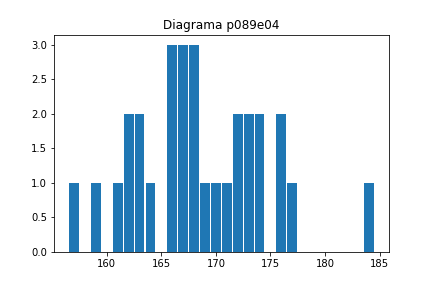
\includegraphics[width=1\columnwidth]{p089e04}   \end{solution} \part[1] Calcular los parámetros de centralización  \begin{solution}   {'media': 168.5, 'mediana': 168.0, 'moda': ModeResult(mode=array([166]), count=array([3]))}   \end{solution} \part[1] Calcular los parámetros de posición P70, Q1, Q3, D4  \begin{solution}   {'P70': 172.0, 'Q1': 164.5, 'Q3': 172.75, 'D4': 167.0}   \end{solution} \part[1] Calcular los parámetros de dispersión  \begin{solution}   {'rango': 27, 'varianza': 34.31666666666667, 'desviación típica': 5.85804290413331, 'coeficiente variación': 0.0347658332589514}   \end{solution}
        \end{parts}
        \end{multicols}
        \question p090e06 - La medida del tórax de una muestra de varones se distribuye: \\\begin{tabular}{rlr}
\hline
    & Duración                    &   Cantidad \\
\hline
  0 & $\left[79.5, 85.5\right)$   &          4 \\
  1 & $\left[85.5, 91.5\right)$   &          8 \\
  2 & $\left[91.5, 97.5\right)$   &         12 \\
  3 & $\left[97.5, 103.5\right)$  &         20 \\
  4 & $\left[103.5, 109.5\right)$ &          9 \\
  5 & $\left[109.5, 115.5\right)$ &          5 \\
  6 & $\left[115.5, 121.5\right)$ &          2 \\
\hline
\end{tabular}
        \begin{multicols}{1} 
        \begin{parts} \part[1] Haz una tabla de frecuencias  \begin{solution}   \begin{tabular}{rrrrrrrrrr}
\hline
    &   lim\_inf &   lim\_sup &   x\_i &   f\_i &   F\_i &       h\_i &         H\_i &   x\_if\_i &   x\^{}2\_if\_i \\
\hline
  0 &      79.5 &      85.5 &  82.5 &     4 &     4 & 0.0666667 &   0.0666667 &    330   &    27225   \\
  1 &      85.5 &      91.5 &  88.5 &     8 &    12 & 0.133333  &   0.2       &    708   &    62658   \\
  2 &      91.5 &      97.5 &  94.5 &    12 &    24 & 0.2       &   0.4       &   1134   &   107163   \\
  3 &      97.5 &     103.5 & 100.5 &    20 &    44 & 0.333333  &   0.733333  &   2010   &   202005   \\
  4 &     103.5 &     109.5 & 106.5 &     9 &    53 & 0.15      &   0.883333  &    958.5 &   102080   \\
  5 &     109.5 &     115.5 & 112.5 &     5 &    58 & 0.0833333 &   0.966667  &    562.5 &    63281.2 \\
  6 &     115.5 &     121.5 & 118.5 &     2 &    60 & 0.0333333 &   1         &    237   &    28084.5 \\
  7 &     nan   &     nan   & nan   &    60 &   nan & 1         & nan         &   5940   &   592497   \\
\hline
\end{tabular}   \end{solution} \part[1] Calcula media, la varianza, la desviación típica y el coeficiente de variación  \begin{solution}   {'media': 99.0, 'varianza': 73.95000000000073, 'desviación típica': 8.59941858499752, 'coeficiente de variación': 0.0868628139898739}   \end{solution}
        \end{parts}
        \end{multicols}
        \question p090e07 - En una consulta médica la distribución de pacientes por su edad ha sido, en la última semana, la siguiente:\\\begin{tabular}{rlr}
\hline
    & Duración              &   Cantidad \\
\hline
  0 & $\left[15, 23\right)$ &          3 \\
  1 & $\left[23, 31\right)$ &          4 \\
  2 & $\left[31, 39\right)$ &          5 \\
  3 & $\left[39, 47\right)$ &          8 \\
  4 & $\left[47, 55\right)$ &         10 \\
  5 & $\left[55, 63\right)$ &         12 \\
  6 & $\left[63, 71\right)$ &         15 \\
  7 & $\left[71, 79\right)$ &         12 \\
  8 & $\left[79, 87\right)$ &          6 \\
\hline
\end{tabular}
        \begin{multicols}{1} 
        \begin{parts} \part[1] Haz una tabla de frecuencias  \begin{solution}   \begin{tabular}{rrrrrrrrrr}
\hline
    &   lim\_inf &   lim\_sup &   x\_i &   f\_i &   F\_i &       h\_i &         H\_i &   x\_if\_i &   x\^{}2\_if\_i \\
\hline
  0 &        15 &        23 &    19 &     3 &     3 & 0.04      &   0.04      &       57 &       1083 \\
  1 &        23 &        31 &    27 &     4 &     7 & 0.0533333 &   0.0933333 &      108 &       2916 \\
  2 &        31 &        39 &    35 &     5 &    12 & 0.0666667 &   0.16      &      175 &       6125 \\
  3 &        39 &        47 &    43 &     8 &    20 & 0.106667  &   0.266667  &      344 &      14792 \\
  4 &        47 &        55 &    51 &    10 &    30 & 0.133333  &   0.4       &      510 &      26010 \\
  5 &        55 &        63 &    59 &    12 &    42 & 0.16      &   0.56      &      708 &      41772 \\
  6 &        63 &        71 &    67 &    15 &    57 & 0.2       &   0.76      &     1005 &      67335 \\
  7 &        71 &        79 &    75 &    12 &    69 & 0.16      &   0.92      &      900 &      67500 \\
  8 &        79 &        87 &    83 &     6 &    75 & 0.08      &   1         &      498 &      41334 \\
  9 &       nan &       nan &   nan &    75 &   nan & 1         & nan         &     4305 &     268867 \\
\hline
\end{tabular}   \end{solution} \part[1] Calcula media, la varianza, la desviación típica y el coeficiente de variación  \begin{solution}   {'media': 57.4, 'varianza': 290.13333333333367, 'desviación típica': 17.0333007175161, 'coeficiente de variación': 0.296747399259862}   \end{solution} \part[1] La edad mas frecuente de los pacientes  \begin{solution}   {'Intervalo modal': '$\\left[63.0, 71.0\\right)$', 'moda': 67.0}   \end{solution} \part[1] El percentil 47  \begin{solution}   {'k': 47, 'N': 75.0, '$L_i$': 55.0, '$f_i$': 12.0, '$F_{i-1}$': 30.0, '$C_i$': 8.0, 'percentil': 58.5}   \end{solution} \part[1] ¿Qué porcentaje de pacientes tenían una edad superior a 60 años?  \begin{solution}   {'valor': 60, 'N': 75.0, '$L_i$': 55.0, '$f_i$': 12.0, '$F_{i-1}$': 30.0, '$C_i$': 8.0, 'Porcentaje': 50.0000000000000}   \end{solution}
        \end{parts}
        \end{multicols}
        \question p90e05 - La realización de una prueba de habilidad motora por parte de 60 niños ha dado los resultados siguientes:15
76
29
35
75
31
18
19
52
23
15
46
73
23
18
81
35
17
19
81
35
27
15
62
15
81
44
18
41
31
63
76
18
45
24
27
31
27
32
32
69
74
45
15
19
18
18
31
29
13
47
17
18
19
30
76
82
77
14
50 
        \begin{multicols}{1} 
        \begin{parts} \part[1] Realiza una tabla de frecuencias  \begin{solution}   \begin{tabular}{rrrrrrr}
\hline
   x\_i &   f\_i &   F\_i &       r\_i &      R\_i &      \%\_i &     \%A\_i \\
\hline
    15 &    20 &    20 & 0.333333  & 0.333333 & 33.3333  &  33.3333 \\
    25 &     8 &    28 & 0.133333  & 0.466667 & 13.3333  &  46.6667 \\
    35 &    10 &    38 & 0.166667  & 0.633333 & 16.6667  &  63.3333 \\
    45 &     6 &    44 & 0.1       & 0.733333 & 10       &  73.3333 \\
    55 &     2 &    46 & 0.0333333 & 0.766667 &  3.33333 &  76.6667 \\
    65 &     3 &    49 & 0.05      & 0.816667 &  5       &  81.6667 \\
    75 &     7 &    56 & 0.116667  & 0.933333 & 11.6667  &  93.3333 \\
    85 &     4 &    60 & 0.0666667 & 1        &  6.66667 & 100      \\
\hline
\end{tabular}   \end{solution} \part[1] Realiza un diagrama de barras y un polígono de frecuencias  \begin{solution}   \\ 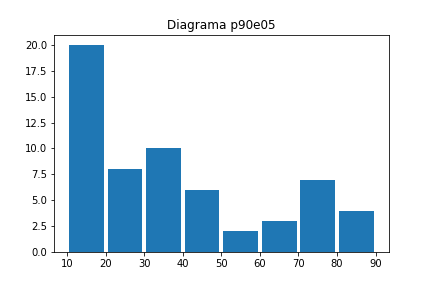
\includegraphics[width=1\columnwidth]{p90e05}   \end{solution} \part[1] Calcular los parámetros de centralización  \begin{solution}   {'media': 38.166666666666664, 'mediana': 35.0, 'moda': ModeResult(mode=array([15.]), count=array([20]))}   \end{solution} \part[1] Calcular los parámetros de posición  \begin{solution}   {'Q1': 15.0, 'Q3': 55.0}   \end{solution} \part[1] Calcular los parámetros de dispersión  \begin{solution}   {'rango': 70.0, 'varianza': 558.3055555555554, 'desviación típica': 23.6284903359388, 'coeficiente variación': 0.619087083037699}   \end{solution} \part[1] Realiza una tabla de frecuencias  \begin{solution}   \begin{tabular}{rrrrrrr}
\hline
   x\_i &   f\_i &   F\_i &       r\_i &      R\_i &      \%\_i &     \%A\_i \\
\hline
    15 &    20 &    20 & 0.333333  & 0.333333 & 33.3333  &  33.3333 \\
    25 &     8 &    28 & 0.133333  & 0.466667 & 13.3333  &  46.6667 \\
    35 &    10 &    38 & 0.166667  & 0.633333 & 16.6667  &  63.3333 \\
    45 &     6 &    44 & 0.1       & 0.733333 & 10       &  73.3333 \\
    55 &     2 &    46 & 0.0333333 & 0.766667 &  3.33333 &  76.6667 \\
    65 &     3 &    49 & 0.05      & 0.816667 &  5       &  81.6667 \\
    75 &     7 &    56 & 0.116667  & 0.933333 & 11.6667  &  93.3333 \\
    85 &     4 &    60 & 0.0666667 & 1        &  6.66667 & 100      \\
\hline
\end{tabular}   \end{solution} \part[1] Realiza un diagrama de barras y un polígono de frecuencias  \begin{solution}   \\ 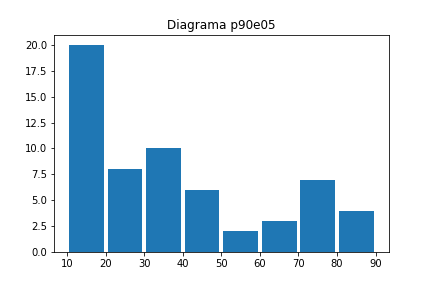
\includegraphics[width=1\columnwidth]{p90e05}   \end{solution} \part[1] Calcular los parámetros de centralización  \begin{solution}   {'media': 38.166666666666664, 'mediana': 35.0, 'moda': ModeResult(mode=array([15.]), count=array([20]))}   \end{solution} \part[1] Calcular los parámetros de posición  \begin{solution}   {'Q1': 15.0, 'Q3': 55.0}   \end{solution} \part[1] Calcular los parámetros de dispersión  \begin{solution}   {'rango': 70.0, 'varianza': 558.3055555555554, 'desviación típica': 23.6284903359388, 'coeficiente variación': 0.619087083037699}   \end{solution}
        \end{parts}
        \end{multicols}
        
    \end{questions}
    \end{document}
    